\documentclass[a4paper,12pt]{article}
\usepackage[english,ukrainian,russian]{babel}
\linespread{1,2}
\usepackage{ucs}
\usepackage[utf8]{inputenc}
\usepackage[T2A]{fontenc}
\usepackage[paper=portrait,pagesize]{typearea}
\usepackage{amsmath}
\usepackage{bigints}
\usepackage{amsfonts}
\usepackage{graphicx}
\usepackage{amssymb}
\usepackage{cancel}
\usepackage{gensymb}
\usepackage{multirow}
\usepackage{rotate} 
\usepackage{pdflscape}
\usepackage{bigstrut}
\usepackage[pageanchor]{hyperref}
\usepackage{svg}
\usepackage{chngpage}
\newcommand{\dx}{\textbf{d}x}
\newcommand{\dt}{\textbf{d}t}
\newcommand{\du}{\textbf{d}u}
\newcommand{\dv}{\textbf{d}v}
\newcommand{\dy}{\textbf{d}y}
\newcommand{\ds}{\textbf{d}s}
\newcommand{\dz}{\textbf{d}z}
\newcommand{\dr}{\textbf{d}r}
\newcommand{\arch}{\textrm{arcch}}
\newcommand{\arsh}{\textrm{arcsh}}
\newcommand{\dint}{\displaystyle\int}
\newcommand{\doint}{\displaystyle\oint}
\newcommand\tab[1][1cm]{\hspace*{#1}}
\newcommand{\dsum}{\displaystyle\sum}
\newcommand{\RomanNumeralCaps}[1]{\MakeUppercase{\romannumeral #1}}
\usepackage[left=20mm, top=20mm, right=15mm, bottom=15mm, nohead, nofoot]{geometry}
\newcommand{\ri}{R_i}
\newcommand{\re}{R_e}
\newcommand{\uo}{U_0}
\newcommand{\ik}{I_{kz}}
\newcommand{\po}{P_0}
\newcommand{\pio}{P_i}
\newcommand{\pe}{P_e}





\begin{document}
	\begin{center}
		{\Large \bfseries \textsc{Розрахункова робота}}\\
		\hrulefill\\
		\Large \textsc{ФІ-12 Завалій Олександр\\ Варіант №5}
	\end{center}
	
	\begin{table}[h!]
		\resizebox{.4\textwidth}{!}{%
			\begin{tabular}{l|l}
				\multicolumn{1}{c|}{\textbf{Дано:}}           & \multirow{3}{*}{$\doint\vec{E}\vec{n}\ds=\dfrac{Q}{\varepsilon_0}$} \\
				$\rho(r)=\rho_0\cos\dfrac{\pi x}{2d}$ &                   \\ 
				$\sigma=0,5$ нКл/м$^2$ &                   \\ 
				$\rho_0=50$ нКл/м$^3$ &                  \\ 
				$d=5$см$=0.05$м &                   \\ \cline{1-1}        
				$E_{x}(x),\:\varphi(x) - ?$                &             \\      
			\end{tabular}%
		}
	\end{table}
	
	\begin{figure}[h!]
		\begin{minipage}[h]{0.5\linewidth}
			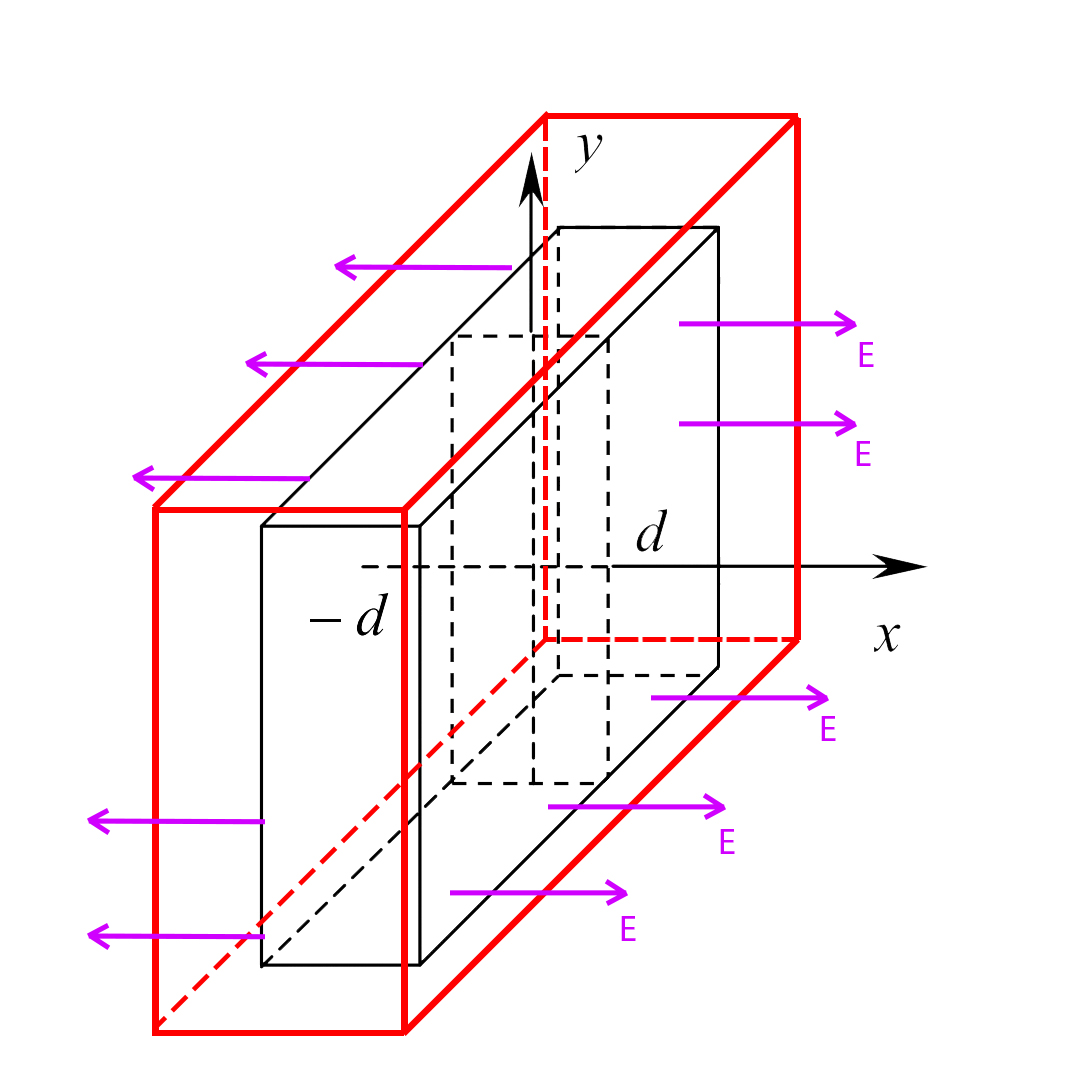
\includegraphics[width=1\linewidth]{Prt sc/big_1.jpg}
			\label{Figure_1_1}
			\caption{Зовнішня математична поверхня.}
		\end{minipage}
		\begin{minipage}[h]{0.5\linewidth}
			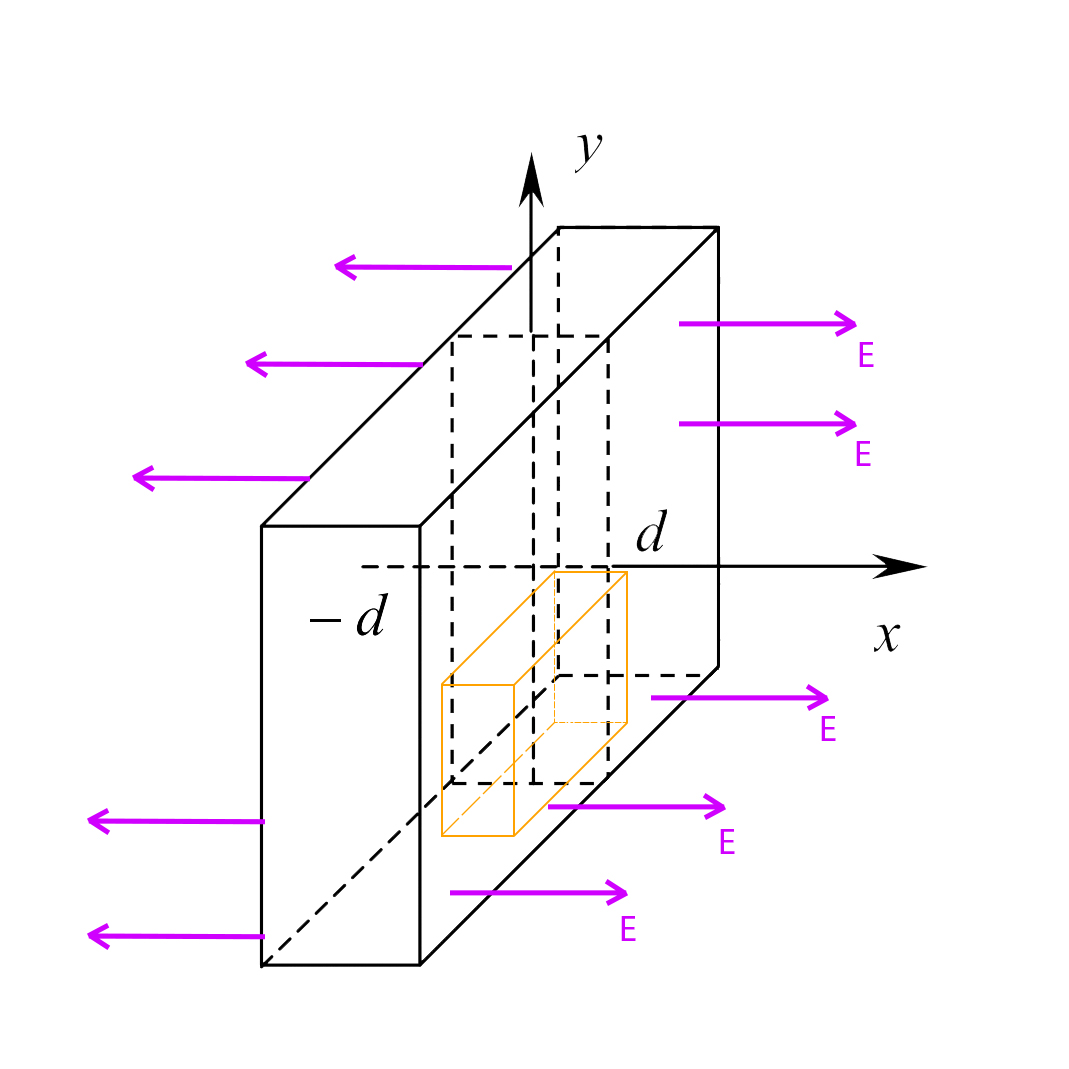
\includegraphics[width=1\linewidth]{Prt sc/small_2.jpg}
			\label{Figure_1_2}
			\caption{Внутрішня математична поверхня.}
		\end{minipage}
	\end{figure}
\newpage
	\begin{center}
		\section*{Розв'язання}
	\end{center}
	\begin{center}
		\fbox{$\doint\vec{E}\ds=\vec{E}\doint\ds=\vec{E}\cdot S=\dfrac{Q}{\varepsilon_0}\Rightarrow\vec{E}=\dfrac{Q}{\varepsilon_0\cdot S};\:\:\: Q_{ex}=\dint\limits_{-d}^{d}\rho\dv+2\sigma S;\:\:\:\dv=S\dx;\:\:\:\varphi=-\dint\vec{E}\dr+C$}
	\end{center}
	\begin{center}
		\textbf{Заряд Q}
	\end{center}
	\begin{enumerate}
		\item[\RomanNumeralCaps{1})] 
		$Q_{ex}=\dint\limits_{-d}^{d}\rho_0S\cos\dfrac{\pi x}{2d}\dx+2\sigma S= \dfrac{2d\rho_0S}{\pi}\cdot\bigg(\sin\dfrac{\pi x}{2d}\bigg)\bigg|_{-d}^{d}+2\sigma S=\dfrac{4d\rho_0S}{\pi}+2\sigma S$
		\item[\RomanNumeralCaps{2})]
		$Q_{in}=\dint\limits_{-x}^{x}\rho_0S\cos\dfrac{\pi x}{2d}\dx=\dfrac{2d\rho_0S}{\pi}\cdot\bigg(\sin\dfrac{\pi x}{2d}\bigg)\bigg|_{-x}^{x}=\dfrac{4d\rho_0S\sin(\frac{\pi x}{2d})}{\pi}$
	\end{enumerate}
	\begin{center}
		\textbf{Напруженість електричного поля $E$}
	\end{center}
	\begin{enumerate}
		\item[\RomanNumeralCaps{1})]
		$E_{ex}=\dfrac{4d\rho_0S+2\pi\sigma S}{\pi\varepsilon_0S}=\dfrac{4d\rho_0+2\pi\sigma}{\pi\varepsilon_0}\cdot\dfrac{x}{|x|}$
		\item[\RomanNumeralCaps{2})]
		$E_{in}=\dfrac{4d\rho_0\cancel{S}\sin(\frac{\pi x}{2d})}{\pi\varepsilon_0 \cancel{S}}=\dfrac{4d\rho_0\sin(\frac{\pi x}{2d})}{\pi\varepsilon_0}$
	\end{enumerate}
	\begin{center}
		\textbf{Потенціал поля $\varphi$}
	\end{center}
	\begin{enumerate}
		\item[\RomanNumeralCaps{1})]
		$\varphi_{ex}=-\dint\bigg(\dfrac{4d\rho_0+2\pi\sigma}{\pi\varepsilon_0}\bigg)\dx=-\dfrac{x(4d\rho_0+2\pi\sigma)}{\pi\varepsilon_0}+C$
		\item[\RomanNumeralCaps{2})]
		$\varphi_{in}=-\dfrac{4d\rho_0}{\pi\varepsilon_0}\cdot\dint\sin\dfrac{\pi x}{2d}\dx=\dfrac{8d^2\rho_0\cos(\frac{\pi x}{2d})}{\pi^2\varepsilon_0}+C$
		\begin{enumerate}
			\item[a)] $\varphi_{in}(0)=0$ \\
			$\\ \dfrac{8d^2\rho_0\cdot1}{\pi^2\varepsilon_0}+C=0\Rightarrow C=-\dfrac{8d^2\rho_0}{\pi^2\varepsilon_0}$
			\item[b)] $\varphi_{in}(d)=\varphi_{ex}(d)$ \\
			$\\ \dfrac{8d^2\rho_0\cos(\frac{\pi \cancel{d}}{2\cancel{d}})}{\pi^2\varepsilon_0}-\dfrac{8d^2\rho_0}{\pi^2\varepsilon_0}=-\dfrac{d(4d\rho_0+2\pi\sigma)}{\pi\varepsilon_0}+C \Rightarrow C=\dfrac{d(4d\rho_0+2\pi\sigma)}{\pi\varepsilon_0}-\dfrac{8d^2\rho_0}{\pi^2\varepsilon_0}$\\
			$\\C=\dfrac{4d^2\pi\rho_0+2\pi^2d\sigma-8d^2\rho_0}{\pi^2\varepsilon_0}=\dfrac{2d(2d\pi\rho_0+\pi^2\sigma-4d\rho_0)}{\pi^2\varepsilon_0}\Rightarrow$
		\end{enumerate}
	\end{enumerate}
	
\newpage
	\begin{enumerate}
		\item[\RomanNumeralCaps{3})]$\varphi_{ex}=-\dfrac{x(4d\rho_0+2\pi\sigma)}{\pi\varepsilon_0}+\dfrac{2d(2d\pi\rho_0+\pi^2\sigma-4d\rho_0)}{\pi^2\varepsilon_0}$\\
		\item[\RomanNumeralCaps{4})]$\varphi_{in}=\dfrac{8d^2\rho_0\cos(\frac{\pi x}{2d})}{\pi^2\varepsilon_0}-\dfrac{8d^2\rho_0}{\pi^2\varepsilon_0}$
	\end{enumerate}
	
	\begin{figure}[h!]
		\centering
		\begin{minipage}[h]{0.55\linewidth}
			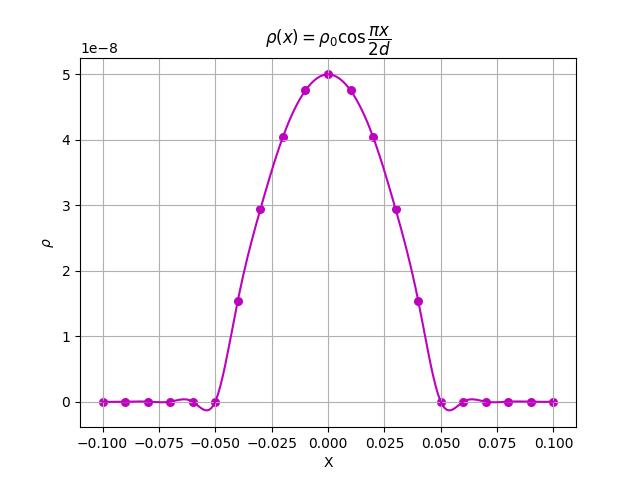
\includegraphics[width=1\linewidth]{Prt sc/Figure_1.jpeg} 
		\end{minipage}
		%\caption{C.}
		\begin{minipage}[h]{0.55\linewidth}
			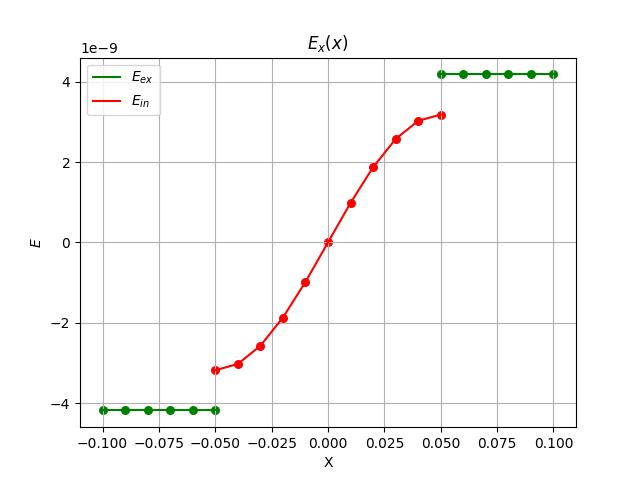
\includegraphics[width=1\linewidth]{Prt sc/Figure_2.jpeg}
		\end{minipage}
		%\caption{B.}
		\begin{minipage}[h]{0.55\linewidth}
			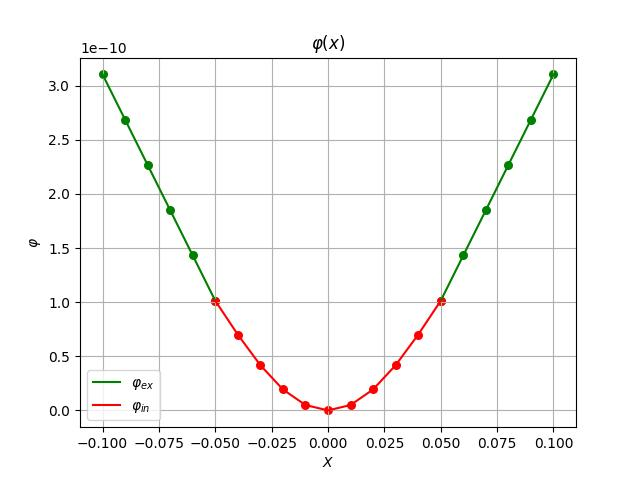
\includegraphics[width=1\linewidth]{Prt sc/Figure_3.jpeg}
		\end{minipage}
		%\caption{C.}
	\end{figure}
	
	
	
	
	
	
	
	
	
	
	
	
	
	
	
\end{document}